\chapter{Metodología}
\chaptermark{Metodología}
\label{metodologia}

En este capítulo se detalla el diseño experimental utilizado para modelar la dinámica de las transiciones del sueño. La metodología se estructura en cinco fases secuenciales: (1) construcción de un dataset unificado de sujetos sanos, (2) determinación de la escala temporal óptima del token, (3) aprendizaje de representaciones vectoriales mediante Word2Vec, (4) análisis de estabilidad matricial por ciclos, y (5) modelado predictivo recurrente con una red LSTM. La Figura \ref{fig:pipeline} resume este flujo de trabajo de principio a fin.

\begin{figure}[htbp]
    \centering
    
\includegraphics[width=\textwidth]{pipeline_general.png}
    \caption{Flujo general del proyecto: las tres fuentes de registros se unifican en una sola cohorte, se tokenizan mediante ventaneo deslizante y alimentan los modelos de análisis.}
    \label{fig:pipeline}
\end{figure}

\section{Descripción del Dataset}

Para construir un modelo robusto del sueño sano y, a la vez, disponer de potencia estadística suficiente, se unificaron tres fuentes independientes de registros polisomnográficos de personas sanas. La unificación se realiza de forma idempotente en el primer notebook del proyecto, que homogeneiza los identificadores, la codificación de fases y la demografía disponible.

\subsection{Población y Muestra}

La cohorte de sujetos sanos se compone de \textbf{127 pacientes}, provenientes de tres fuentes:

\begin{itemize}
    \item \textbf{CAP} (\textit{CAP Sleep Database}): 16 sujetos sanos.
    \item \textbf{Sleep-EDF} (\textit{Sleep Cassette}): 82 noches, restringidas a participantes de 65 años o menos.
    \item \textbf{SCO} (\textit{Scoring}): 29 registros del laboratorio interno.
\end{itemize}

En conjunto, la cohorte sana reúne \textbf{112\,809 épocas} de 30 segundos, equivalentes a \textbf{940.1 horas} de sueño. La Tabla \ref{tab:dataset_unificado} resume su composición. Los hipnogramas fueron estadificados manualmente por expertos siguiendo reglas estándar \citep{rechtschaffen1968manual}, con ventanas temporales (épocas) de \textbf{30 segundos}.

\begin{table}[htbp]
\centering
\caption{Composición del dataset unificado de sujetos sanos.}
\label{tab:dataset_unificado}
\begin{tabular}{lrrrr}
\hline
\textbf{Fuente} & \textbf{Pacientes} & \textbf{Épocas} & \textbf{Horas} & \textbf{Edad media} \\
\hline
CAP   & 16  & 15\,947  & 132.9 & 32.2 \\
EDF   & 82  & 70\,410  & 586.8 & 41.9 \\
SCO   & 29  & 26\,452  & 220.4 & --   \\
\hline
\textbf{Total} & \textbf{127} & \textbf{112\,809} & \textbf{940.1} & \textbf{40.3} \\
\hline
\end{tabular}
\end{table}

La distribución de fases, edades y duración por fuente se presenta en el Capítulo \ref{resultados}. La fuente SCO no dispone de metadatos demográficos, por lo que sus campos de sexo y edad quedan vacíos.

\subsection{Homogeneización entre Fuentes}

Cada fuente fue preprocesada para garantizar comparabilidad: en CAP se fusionaron las etapas S3 y S4 en sueño de ondas lentas (SWS) según el criterio de Rechtschaffen \& Kales; en Sleep-EDF se truncaron los tramos prolongados de vigilia previa y posterior al sueño y se filtró por edad ($\leq 65$ años); y en SCO se utilizó la estadificación limpia validada por expertos. Tras la unificación, los identificadores quedan prefijados por fuente (\texttt{CAP\_*}, \texttt{EDF\_*}, \texttt{SCO\_*}) y todas las fases comparten una única codificación.

\section{Preprocesamiento y Codificación}

\subsection{Sistema de Clasificación Unificado}

Cada fuente empleaba originalmente su propia codificación de estadios. Durante la unificación, todas las fases se mapearon a una codificación numérica común (0--5) mostrada en la Tabla \ref{tab:codificacion_original}.

\begin{table}[htbp]
\centering
\caption{Codificación unificada de estados de sueño en el dataset.}
\label{tab:codificacion_original}
\begin{tabular}{cl}
\hline
\textbf{Código} & \textbf{Estado} \\
\hline
0 & Vigilia (W) \\
1 & Sueño Ligero Etapa 1 (S1) \\
2 & Sueño Ligero Etapa 2 (S2) \\
3 & Sueño de Ondas Lentas (SWS = S3 + S4) \\
4 & Sueño REM \\
5 & Sin Clasificar (incluye Movimiento) \\
\hline
\end{tabular}
\end{table}

\subsection{Definición del Espacio de Estados}

La fusión de las etapas \textbf{S3 y S4} en una sola categoría de sueño de ondas lentas (SWS) se aplica en origen, dado que ambas representan sueño profundo delta y la distinción entre ellas es difusa en términos de dinámica de transición macroscópica. Las épocas \textbf{Sin Clasificar} (código 5, que agrupa movimiento y etiquetas ausentes) se tratan como ruido y se excluyen del cálculo de matrices de transición.

El ``vocabulario'' de fases del modelo queda constituido por \textbf{5 estados fundamentales}:
\begin{equation}
    \mathcal{S} = \{ \text{W}, \text{S1}, \text{S2}, \text{SWS}, \text{REM} \}
    \label{eq:vocabulario}
\end{equation}

La Tabla \ref{tab:codificacion_simplificada} resume el mapeo aplicado en cada fuente.

\begin{table}[htbp]
\centering
\caption{Mapeo de las etapas originales al espacio de estados unificado.}
\label{tab:codificacion_simplificada}
\small\setlength{\tabcolsep}{5pt}%
\begin{tabular}{cll}
\hline
\textbf{Código} & \textbf{Estado Unificado} & \textbf{Nota} \\
\hline
0 & Vigilia (W) & \\
1 & S1 & \\
2 & S2 & \\
3 & SWS & fusión de S3 y S4 \\
4 & REM & \\
5 & Sin Clasificar & movimiento y etiquetas ausentes (excluido) \\
\hline
\end{tabular}
\end{table}

\section{Determinación de la Escala Temporal}

Un problema central al aplicar modelos de n-gramas a series temporales fisiológicas es la elección del tamaño de ventana $N$. Una selección arbitraria puede cortar procesos biológicos de distinta escala o introducir artefactos estadísticos. En lugar de fijar $N$ a priori, se eligió de forma empírica sobre la cohorte unificada de 127 pacientes combinando tres criterios independientes.

\subsection{Criterios de Selección}

Para cada candidato de $N$ se construyen todos los n-gramas del corpus y se evalúan:

\begin{enumerate}
    \item \textbf{Ley de Zipf ($\beta$):} se ordenan los n-gramas por frecuencia descendente y se ajusta por mínimos cuadrados la recta $\log_{10}(\text{frecuencia}) = a - \beta \log_{10}(\text{rango})$. Una distribución de tipo lenguaje natural tiene $\beta \approx 1$.
    \item \textbf{Calidad del ajuste ($R^2$):} mide cuán limpia es la ley de potencia. Un $R^2$ alto indica una recta log-log bien definida y no ruido.
    \item \textbf{Cobertura de los bloques de S2:} la fase 2 aparece en bloques de épocas consecutivas. Se mide qué fracción de esos bloques tiene longitud mayor o igual a $N$; así, una ventana que cabe dentro del bloque típico captura una unidad fisiológica completa.
\end{enumerate}

\subsection{Barrido y Criterio Combinado}

Se realizó un barrido amplio de $N$ (de 1 hasta 100) para caracterizar el comportamiento global, y un ranking fino sobre los candidatos $N \in \{5,6,7,8,9,10,12,15\}$. El detalle numérico se presenta en el Capítulo \ref{resultados}; aquí se resume la decisión.

El valor de $\beta$ crece hasta $N=2$ y luego decrece monótonamente, cruzando $\beta = 1$ entre $N=8$ y $N=10$. Si se atendiera únicamente a $|\beta - 1|$, el ganador sería $N=10$. Sin embargo, ese criterio aislado ignora la calidad del ajuste y la coherencia fisiológica. Al combinar los tres criterios en un ranking por posición media, el mejor balance lo obtiene:

\begin{equation}
    N = 6 \text{ épocas} \quad (\approx 3 \text{ minutos})
    \label{eq:ventana}
\end{equation}

En $N=6$ el ajuste log-log alcanza su mayor calidad ($R^2 = 0.977$) y la ventana sigue cabiendo dentro de casi la mitad de los bloques de S2 (cobertura del 47.3\%), mientras que $\beta = 1.60$ se mantiene en un rango compatible con estructura de lenguaje. Es decir, $N=6$ no minimiza la distancia a Zipf, pero es el tamaño que mejor concilia los tres criterios simultáneamente. Este valor define el token para el resto del análisis vectorial.

\section{Entrenamiento de Embeddings (Word2Vec)}

\subsection{Tokenización Temporal (N-gramas)}

A diferencia del análisis estadístico tradicional que trata cada época como un punto independiente, este estudio define la unidad mínima de análisis (token) como una \textbf{secuencia temporal de 6 épocas consecutivas}.

Cada token se codifica como una cadena del tipo \texttt{a-b-c-d-e-f}, donde cada letra representa el estado simplificado de una época. Por ejemplo, el token \texttt{2-2-2-2-2-3} representa una ventana donde predomina S2 y la última época corresponde a SWS.

\subsection{Generación del Corpus y Selección del Stride}

El corpus de entrenamiento se generó mediante un \textbf{ventaneo deslizante (sliding window)} con los siguientes parámetros:
\begin{itemize}
    \item \textbf{Tamaño de ventana:} $N = 6$ épocas
    \item \textbf{Paso (stride):} 1 época (máximo solapamiento)
\end{itemize}

\begin{figure}[htbp]
    \centering
    
\includegraphics[width=\textwidth]{ventana_deslizante.png}
    \caption{Ventaneo deslizante con $N=6$ y paso de una época. Cada token agrupa seis épocas consecutivas y la ventana avanza de una en una, de modo que tokens contiguos comparten cinco de sus seis épocas.}
    \label{fig:ventana_deslizante}
\end{figure}

\textbf{Justificación del Stride:} Se adoptó un paso de una sola época (solapamiento máximo) en lugar de un ventaneo sin solapamiento. La razón es doble. Primero, la \textbf{robustez estadística}: con paso 1 cada noche aporta tantas ventanas como épocas tiene, lo que multiplica el volumen del corpus y permite estimar representaciones estables incluso para 6-gramas poco frecuentes; un paso igual a $N$ reduciría el corpus en un factor de seis y dejaría sin soporte a buena parte del vocabulario. Segundo, la \textbf{coherencia fisiológica}: el sueño es un proceso progresivo y continuo, de modo que ventanas que comparten cinco de sus seis épocas describen estados vecinos en una trayectoria suave; preservar ese solapamiento mantiene la continuidad de las transiciones, mientras que un ventaneo disjunto fragmentaría la secuencia y borraría los cambios graduales entre fases. El costo conocido de esta decisión es la autocorrelación entre ventanas consecutivas: como tokens contiguos comparten cinco de sus seis épocas, las $\sim$110\,000 ventanas \textbf{no son observaciones independientes}, por lo que el \textit{tamaño efectivo de muestra} es sustancialmente menor que el conteo bruto y los intervalos de confianza ingenuos subestimarían la incertidumbre. Asumimos este sesgo como contrapartida del mayor tamaño y suavidad del corpus; para verificar que las conclusiones no son un artefacto del solapamiento, el análisis clave se repite con un paso disjunto ($\text{stride}=N$) ---que elimina la autocorrelación entre ventanas a costa de un corpus seis veces menor---, cuyo resultado se reporta en la Sección \ref{sec:deslizador_stride}.

El corpus unificado contiene del orden de \textbf{110\,000 ventanas} de 6 épocas. Tras filtrar los hápax (tokens con frecuencia menor a 2), el vocabulario de 6-gramas quedó en \textbf{1\,503 tokens}. El token dominante es \texttt{2-2-2-2-2-2} (S2 sostenido), coherente con que S2 ocupa cerca de la mitad del tiempo nocturno.

\subsection{Arquitectura del Modelo}

Se implementó el modelo \textbf{Word2Vec Skip-Gram} \citep{mikolov2013efficient} en PyTorch (optimizador Adam, $\text{lr}=0.01$, función de pérdida de entropía cruzada). A lo largo del trabajo se entrenaron \textbf{tres variantes} del modelo según el análisis: una sobre \textbf{unigramas} (para la validación topológica de las fases individuales) y dos sobre \textbf{6-gramas} que se diferencian únicamente en el umbral de frecuencia mínima (\texttt{min\_freq}). La Tabla \ref{tab:hiperparametros_w2v} las documenta de forma explícita para garantizar la trazabilidad.

\begin{table}[htbp]
\centering
\caption{Hiperparámetros de las tres variantes de Word2Vec entrenadas. Comparten optimizador (Adam, lr~0.01), tamaño de batch (512) y semilla (42).}
\label{tab:hiperparametros_w2v}
\footnotesize\setlength{\tabcolsep}{4pt}%
\begin{tabular}{lccc}
\hline
\textbf{Parámetro} & \textbf{Unigramas} & \textbf{6-gramas} & \textbf{6-gramas (mf1)} \\
\hline
Dimensión del embedding & 24 & 32 & 32 \\
Ventana contextual & 3 & 1 & 1 \\
Épocas de entrenamiento & 20 & 30 & 30 \\
Frecuencia mínima (\texttt{min\_freq}) & 2 & 2 & 1 \\
Tamaño del vocabulario & 6 & 1\,503 & 2\,817 \\
Uso principal & Topología 1g & Topología 6g & Deslizador y LSTM \\
\hline
\end{tabular}
\end{table}

La ventana contextual de 1 en los modelos de 6-gramas se justifica porque cada token ya encapsula 6 épocas de contexto temporal; contextos más amplios serían redundantes (en unigramas, donde el token es una sola época, se usa ventana 3).

\textbf{Nota sobre la variante \texttt{mf1}.} Los dos experimentos centrales basados en 6-gramas ---el \emph{Deslizador} (Sección \ref{sec:deslizador_metodo}) y el modelo recurrente LSTM--- utilizan una variante entrenada con \texttt{min\_freq}=1 (vocabulario de 2\,817 tokens), en lugar del modelo de topología con \texttt{min\_freq}=2 (1\,503 tokens). La razón es que estos análisis recorren secuencias de transición que incluyen 6-gramas poco frecuentes (cercanos a hápax); descartarlos dejaría sin representación a varias ventanas de la trayectoria. El modelo subrogado correspondiente se entrena con el mismo criterio \texttt{min\_freq}=1 sobre la secuencia permutada.

\section{Análisis de Trayectorias: Interpolación de Estados}
\label{sec:deslizador_metodo}

El experimento del \textbf{Deslizador} consiste en observar cómo evoluciona la representación vectorial de una ventana de S2 conforme se infiltran progresivamente épocas de un estado destino (REM o SWS). Procede sobre secuencias sintéticas e ilustra la organización geométrica del espacio de embeddings; la evidencia de anticipación sobre datos reales se aborda después con el modelo recurrente.

\subsection{Diseño del Experimento}

Se construyeron secuencias sintéticas que representan la transición progresiva desde un estado ``puro'' de S2 hacia los estados destino. La Figura \ref{fig:interpolacion} ilustra este proceso de interpolación gradual.

\begin{figure}[htbp]
    \centering
    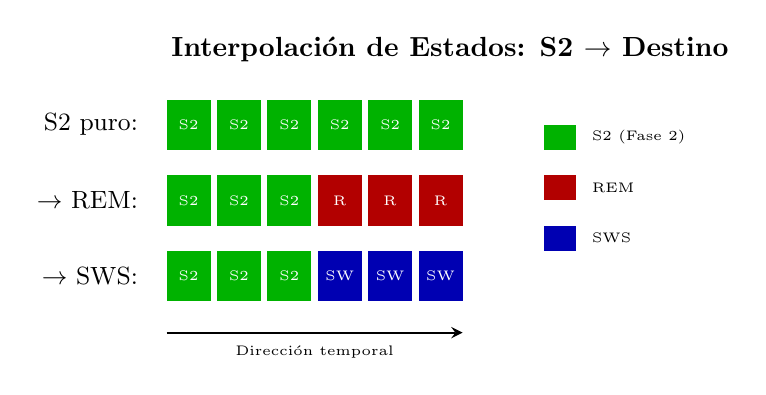
\begin{tikzpicture}[scale=0.8]
        % Título
        \node[font=\bfseries] at (4.5, 3.2) {Interpolación de Estados: S2 $\rightarrow$ Destino};
        
        % Estado inicial S2 puro
        \node[font=\small, anchor=east] at (-0.3, 2) {S2 puro:};
        \foreach \x in {0,...,5} {
            \fill[green!70!black] (\x*0.8, 1.6) rectangle (\x*0.8+0.7, 2.4);
            \node[font=\tiny, white] at (\x*0.8+0.35, 2) {S2};
        }
        
        % Transición hacia REM (rojo)
        \node[font=\small, anchor=east] at (-0.3, 0.8) {$\rightarrow$ REM:};
        \fill[green!70!black] (0, 0.4) rectangle (0.7, 1.2);
        \fill[green!70!black] (0.8, 0.4) rectangle (1.5, 1.2);
        \fill[green!70!black] (1.6, 0.4) rectangle (2.3, 1.2);
        \fill[red!70!black] (2.4, 0.4) rectangle (3.1, 1.2);
        \fill[red!70!black] (3.2, 0.4) rectangle (3.9, 1.2);
        \fill[red!70!black] (4.0, 0.4) rectangle (4.7, 1.2);
        \node[font=\tiny, white] at (0.35, 0.8) {S2};
        \node[font=\tiny, white] at (1.15, 0.8) {S2};
        \node[font=\tiny, white] at (1.95, 0.8) {S2};
        \node[font=\tiny, white] at (2.75, 0.8) {R};
        \node[font=\tiny, white] at (3.55, 0.8) {R};
        \node[font=\tiny, white] at (4.35, 0.8) {R};
        
        % Transición hacia SWS (azul)
        \node[font=\small, anchor=east] at (-0.3, -0.4) {$\rightarrow$ SWS:};
        \fill[green!70!black] (0, -0.8) rectangle (0.7, 0);
        \fill[green!70!black] (0.8, -0.8) rectangle (1.5, 0);
        \fill[green!70!black] (1.6, -0.8) rectangle (2.3, 0);
        \fill[blue!70!black] (2.4, -0.8) rectangle (3.1, 0);
        \fill[blue!70!black] (3.2, -0.8) rectangle (3.9, 0);
        \fill[blue!70!black] (4.0, -0.8) rectangle (4.7, 0);
        \node[font=\tiny, white] at (0.35, -0.4) {S2};
        \node[font=\tiny, white] at (1.15, -0.4) {S2};
        \node[font=\tiny, white] at (1.95, -0.4) {S2};
        \node[font=\tiny, white] at (2.75, -0.4) {SW};
        \node[font=\tiny, white] at (3.55, -0.4) {SW};
        \node[font=\tiny, white] at (4.35, -0.4) {SW};
        
        % Leyenda
        \fill[green!70!black] (6, 1.6) rectangle (6.5, 2);
        \node[font=\tiny, anchor=west] at (6.6, 1.8) {S2 (Fase 2)};
        \fill[red!70!black] (6, 0.8) rectangle (6.5, 1.2);
        \node[font=\tiny, anchor=west] at (6.6, 1) {REM};
        \fill[blue!70!black] (6, 0) rectangle (6.5, 0.4);
        \node[font=\tiny, anchor=west] at (6.6, 0.2) {SWS};
        
        % Flecha de tiempo
        \draw[-stealth, thick] (0, -1.3) -- (4.7, -1.3);
        \node[font=\tiny] at (2.35, -1.6) {Dirección temporal};
    \end{tikzpicture}
    \caption{Diagrama del experimento de Interpolación de Estados. Se construyen secuencias sintéticas que transitan gradualmente desde S2 puro hacia REM (rojo) o SWS (azul), permitiendo medir cómo evoluciona el vector en el espacio latente.}
    \label{fig:interpolacion}
\end{figure}

Formalmente, las secuencias de interpolación se definen como:
\begin{itemize}
    \item \textbf{Estado inicial (S2 puro):} \texttt{2-2-2-2-2-2}
    \item \textbf{Transición hacia REM:} \texttt{2-2-2-2-2-4} $\rightarrow$ \texttt{2-2-2-2-4-4} $\rightarrow$ ... $\rightarrow$ \texttt{4-4-4-4-4-4}
    \item \textbf{Transición hacia SWS:} \texttt{2-2-2-2-2-3} $\rightarrow$ \texttt{2-2-2-2-3-3} $\rightarrow$ ... $\rightarrow$ \texttt{3-3-3-3-3-3}
\end{itemize}

\subsection{Métrica: Distancia Coseno}

Para cada paso de la transición, se calculó la \textbf{Distancia Coseno} entre el vector del estado puro (S2) y el vector de la secuencia en transición:

\begin{equation}
    d_{\cos}(\vec{v}_1, \vec{v}_2) = 1 - \frac{\vec{v}_1 \cdot \vec{v}_2}{\|\vec{v}_1\| \|\vec{v}_2\|}
    \label{eq:distancia_coseno}
\end{equation}

Valores cercanos a 0 indican alta similitud (vectores paralelos); valores cercanos a 2 indican máxima disimilitud (vectores opuestos).

\subsection{Hipótesis de Bifurcación}

Si la Fase 2 posee ``memoria latente'' sobre su destino, las trayectorias hacia REM y SWS deberían \textbf{divergir antes} de que el símbolo destino sea mayoritario en el n-grama. Es decir, el modelo debería detectar la ``intención'' del cerebro antes de que ocurra el cambio clínico visible.

\section{Análisis de Estabilidad: Matrices de Transición de Markov}

Complementando el análisis vectorial, se implementó un enfoque matricial para cuantificar la \textbf{resistencia al cambio} de cada fase.

\subsection{Construcción de Matrices}

Se calcularon \textbf{Matrices de Transición de Markov} de tamaño $5 \times 5$ (una por cada estado del vocabulario simplificado), donde cada elemento $P_{ij}$ representa:

\begin{equation}
    P_{ij} = P(\text{Estado}_{t+1} = j \mid \text{Estado}_t = i)
    \label{eq:prob_transicion}
\end{equation}

\subsection{Análisis Con y Sin Diagonal}

Se generaron dos versiones de las matrices:
\begin{itemize}
    \item \textbf{Con Diagonal:} Incluye la probabilidad de permanencia $P(i|i)$. Revela la \textbf{inercia} o estabilidad de cada fase.
    \item \textbf{Sin Diagonal:} Normaliza las probabilidades excluyendo la auto-transición. Revela \textbf{hacia dónde huye} el cerebro cuando abandona una fase.
\end{itemize}

\subsection{Análisis por Ciclos}

Reconociendo la no-estacionariedad del sueño, las matrices se calcularon de forma independiente para cada \textbf{ciclo ultradiano} (aproximadamente 90 minutos):
\begin{itemize}
    \item Ciclo 1 (0-90 min): Presión homeostática máxima
    \item Ciclo 2 (90-180 min): Transición
    \item Ciclo 3+ (180+ min): Predominancia circadiana
\end{itemize}

Este análisis permite observar cómo evoluciona la \textbf{estabilidad del sueño} a lo largo de la noche.

\section{Validación: Datos Subrogados (Surrogates)}

Para descartar que los patrones observados sean artefactos estadísticos de la frecuencia de los símbolos, se implementó un procedimiento de \textbf{validación con datos subrogados (shuffling temporal)}.

\subsection{Procedimiento}

\begin{enumerate}
    \item Se aleatorizó el orden temporal de las épocas dentro de cada hipnograma, destruyendo la estructura secuencial pero preservando la distribución de frecuencias.
    \item Se repitió el entrenamiento del modelo Word2Vec con los datos revueltos.
    \item Se recalcularon las trayectorias del experimento del ``Deslizador''.
\end{enumerate}

\subsection{Criterio de Éxito}

Si la divergencia entre las trayectorias REM y SWS \textbf{desaparece} en los datos subrogados, entonces la estructura observada en los datos reales es una propiedad \textbf{biológica genuina} y no un artefacto de la distribución estadística.

\section{Modelo de Lenguaje Recurrente (LSTM)}

El experimento del Deslizador examina vectores aislados. Para evaluar si la información secuencial permite \textit{predecir} la dinámica nocturna, se entrenó una red recurrente \textbf{LSTM} como modelo de lenguaje del sueño.

\subsection{Tarea y Arquitectura}

A diferencia de un clasificador que observa un único 6-grama, el LSTM se despliega sobre la \textbf{noche completa}: recibe la secuencia de 6-gramas de toda la noche (cada token codificado con el embedding Word2Vec \textbf{congelado}) y en cada paso predice la \textbf{siguiente época} (W, S1, S2, SWS, REM). Es la tarea de ``predecir la siguiente palabra'' del procesamiento de lenguaje natural, pero con memoria temporal de largo alcance: el estado oculto acumula el historial completo hasta el instante actual. El embedding se mantiene fijo para que la comparación con los modelos basales sea atribuible a la dinámica recurrente y no a un reentrenamiento de las representaciones. La Figura \ref{fig:lstm} ilustra este despliegue paso a paso.

\begin{figure}[htbp]
    \centering
    
\includegraphics[width=\textwidth]{lstm_desplegada.png}
    \caption{Red LSTM desplegada sobre la secuencia de la noche. En cada paso recibe el embedding del 6-grama actual y predice la fase siguiente, propagando el estado de memoria $h_t$ que acumula el historial temporal.}
    \label{fig:lstm}
\end{figure}

Concretamente, la red consta de tres componentes (Tabla \ref{tab:hiperparametros_lstm}): (i)~una capa de \textit{embedding} que asigna a cada índice de 6-grama su vector Word2Vec de 32 dimensiones y que permanece \textbf{congelada} durante todo el entrenamiento; (ii)~una única capa \textbf{LSTM} de 128 unidades ocultas, desplegada sobre la noche completa, que propaga el estado de memoria $h_t$ acumulando el historial hasta el instante actual; y (iii)~una capa lineal que proyecta el estado oculto de cada paso a las cinco fases del sueño. En total se entrenan unos 83\,600 parámetros. El modelo se optimiza con \textbf{entropía cruzada ponderada por la frecuencia inversa de cada clase} ---para contrarrestar el marcado desbalance del sueño, donde la Fase 2 domina y S1 es escasa--- mediante Adam ($\text{lr}=10^{-3}$) sobre lotes de 16 noches, durante un máximo de 40 épocas con \textbf{parada temprana} (paciencia de 6 épocas sobre la exactitud de validación).

\begin{table}[htbp]
\centering
\caption{Arquitectura e hiperparámetros de entrenamiento de la red LSTM.}
\label{tab:hiperparametros_lstm}
\footnotesize\setlength{\tabcolsep}{4pt}%
\begin{tabular}{ll}
\hline
\textbf{Componente / Hiperparámetro} & \textbf{Valor} \\
\hline
Embedding de entrada & Word2Vec 6-gramas (\texttt{mf1}), 32 dim, \textbf{congelado} \\
Capa recurrente & LSTM, 1 capa, 128 unidades ocultas \\
Capa de salida & Lineal, $128 \rightarrow 5$ (una \textit{logit} por fase) \\
Parámetros entrenables & $\approx$83\,600 \\
Función de pérdida & Entropía cruzada ponderada por clase \\
Optimizador & Adam, $\text{lr}=10^{-3}$ \\
Tamaño de lote & 16 noches \\
Épocas (máx.) / parada temprana & 40 / paciencia 6 \\
Semilla & 42 \\
\hline
\end{tabular}
\end{table}

\subsection{Construcción de Secuencias y Partición Sujeto-Disjunta}

Cada noche se transforma en una secuencia de pasos de predicción: en la posición $t$, la entrada es el 6-grama que abarca las épocas $[t-6,\,t-1]$ ---representado por su índice en el vocabulario Word2Vec--- y el objetivo es la fase observada en la época $t$, es decir, la \textbf{siguiente} época. Las escasas posiciones cuyo 6-grama queda fuera de vocabulario (0.09\,\% del total) se descartan.

La partición en entrenamiento y prueba se realiza \textbf{por sujeto}: los 127 pacientes se reparten de forma \textbf{disjunta} en un 80\,\% para entrenamiento (101 sujetos) y un 20\,\% para prueba (26 sujetos), de modo que todas las noches ---y por tanto todas las ventanas--- de un mismo paciente quedan íntegramente en un único conjunto. Esta decisión es deliberada y crítica: puesto que el corpus se genera con solapamiento máximo, en el que ventanas contiguas comparten cinco de sus seis épocas (Figura \ref{fig:ventana_deslizante}), una partición aleatoria por época o por ventana provocaría \textbf{fuga de datos} ---ventanas casi idénticas del mismo sujeto caerían a la vez en entrenamiento y prueba, inflando las métricas precisamente por la autocorrelación inherente al solapamiento---. Al separar por paciente, esa fuga queda excluida por construcción: el modelo se evalúa exclusivamente sobre sujetos que no observó durante el entrenamiento, por lo que las métricas reportadas ---incluida la matriz de confusión--- reflejan la \textbf{generalización a nuevos individuos} y no la memorización de ventanas solapadas.

\subsection{Modelos Basales y Controles}

El desempeño del LSTM se contrasta con dos basales triviales y un control:

\begin{itemize}
    \item \textbf{Persistencia:} predice que la fase siguiente es igual a la actual.
    \item \textbf{Markov de orden 1:} predice la fase más probable dada únicamente la fase actual.
    \item \textbf{Control \textit{shuffled}:} el mismo LSTM entrenado sobre secuencias permutadas dentro de cada paciente, para comprobar si captura orden temporal o solo frecuencias marginales.
\end{itemize}

\subsection{Evaluación Honesta en Transiciones}

Dado que el sueño es altamente persistente (una fase suele repetirse muchas épocas seguidas), la exactitud global premia a quien simplemente ``no cambia''. Por ello se reporta además una métrica restringida a las \textbf{épocas de transición} (aquellas donde la fase efectivamente cambia), que es donde un modelo aporta valor real. Finalmente se analiza la \textbf{bifurcación de S2}: alineando todas las corridas que parten de S2 en el instante $t=0$ y midiendo la probabilidad asignada a SWS y a REM en los pasos previos, se evalúa si el modelo anticipa el destino antes de la transición.

\section{Herramientas y Reproducibilidad}

El análisis se implementó en Python 3.10 utilizando las siguientes bibliotecas:
\begin{itemize}
    \item \textbf{NumPy} y \textbf{Pandas}: Manipulación y procesamiento de datos
    \item \textbf{PyTorch}: Implementación del modelo Word2Vec (Skip-Gram)
    \item \textbf{SciPy}: Cálculo de distancias (similitud coseno)
    \item \textbf{Plotly}: Visualización interactiva 2D y 3D
    \item \textbf{UMAP} \citep{mcinnes2018umap}: Reducción de dimensionalidad para visualización
\end{itemize}

\subsection{Configuración de UMAP para Visualización}

Dado que UMAP es un algoritmo sensible a sus hiperparámetros, documentamos la configuración exacta utilizada para garantizar la reproducibilidad de las visualizaciones:

\begin{table}[htbp]
\centering
\caption{Hiperparámetros de UMAP para la proyección de embeddings.}
\label{tab:hiperparametros_umap}
\begin{tabular}{ll}
\hline
\textbf{Parámetro} & \textbf{Valor} \\
\hline
\texttt{n\_neighbors} & 15 \\
\texttt{min\_dist} & 0.1 \\
\texttt{metric} & cosine \\
\texttt{n\_components} & 2 (para gráficas 2D) \\
\texttt{random\_state} & 42 \\
\hline
\end{tabular}
\end{table}

\textbf{Nota sobre \texttt{n\_neighbors}:} Este parámetro controla el balance entre estructura local y global. Un valor de 15 preserva vecindades cercanas sin perder la topología global del espacio de embeddings. Valores menores (ej. 5) enfatizarían clústeres más compactos pero podrían fragmentar las trayectorias continuas; valores mayores (ej. 50) suavizarían excesivamente la estructura.

El código fuente y los notebooks de análisis están disponibles en el repositorio del proyecto para garantizar la reproducibilidad de los resultados.
